
\chapter{Budowa sprzętowego generatora liczb losowych}
\section{Projektowanie robota}

Proces projektowania robota rozpoczęto od przeanalizowania różnych metod wykonywania rzutu kością.
Ostatecznie, po przeanalizowaniu kilku koncepcji, zdecydowano się na rozwiązanie wykorzystujące obrotowy 
kubek, wewnątrz którego kość porusza się i odbija od ścianek. Taki mechanizm zapewnia losowość rzutu, a 
jednocześnie jest prosty w konstrukcji i intuicyjny w działaniu. Obracający się kubek został 
zaprojektowany tak, aby jego prędkość i czas trwania obrotu można było precyzyjnie kontrolować, co  w założeniu 
pozwala na uzyskanie wiarygodnych wyników przy każdym rzucie. W celach testowych został skonstruowany prototypowy
model robota zbudowany w taki sposób żeby wszystkie jego komponenty były modułowe. Takie rozwiązanie pozwala na 
łatwe podmiany elementów robota bez potrzeby przeprojektowywania całości robota. Przy budowie wykorzystano 
technologię druku 3d, która pozwala na szybkie modyfikacje przy jednoczesnym zachowaniu bardzo wysokiej dokładności
budowy elementów składowych robota.

Pierwszy prototyp robota składał się z metalowych prętów służących za stelaż oraz elementów wydrukowanych na drukarce 3d.
Tymi elementami był: kubek, ramię służące do montażu kubka, uchwyty do prątów oraz płytka mocująca do kamery. Dodatkowo
wykorzystano silnik prądu stałego napędzający kubek oraz sterownik służący do zasilania i sterowania ruchem silnika.

%tu cos nie dziala
% \begin{figure} % [h] oznacza, że obraz będzie wyświetlony "tuż przy" miejscu wywołania
%     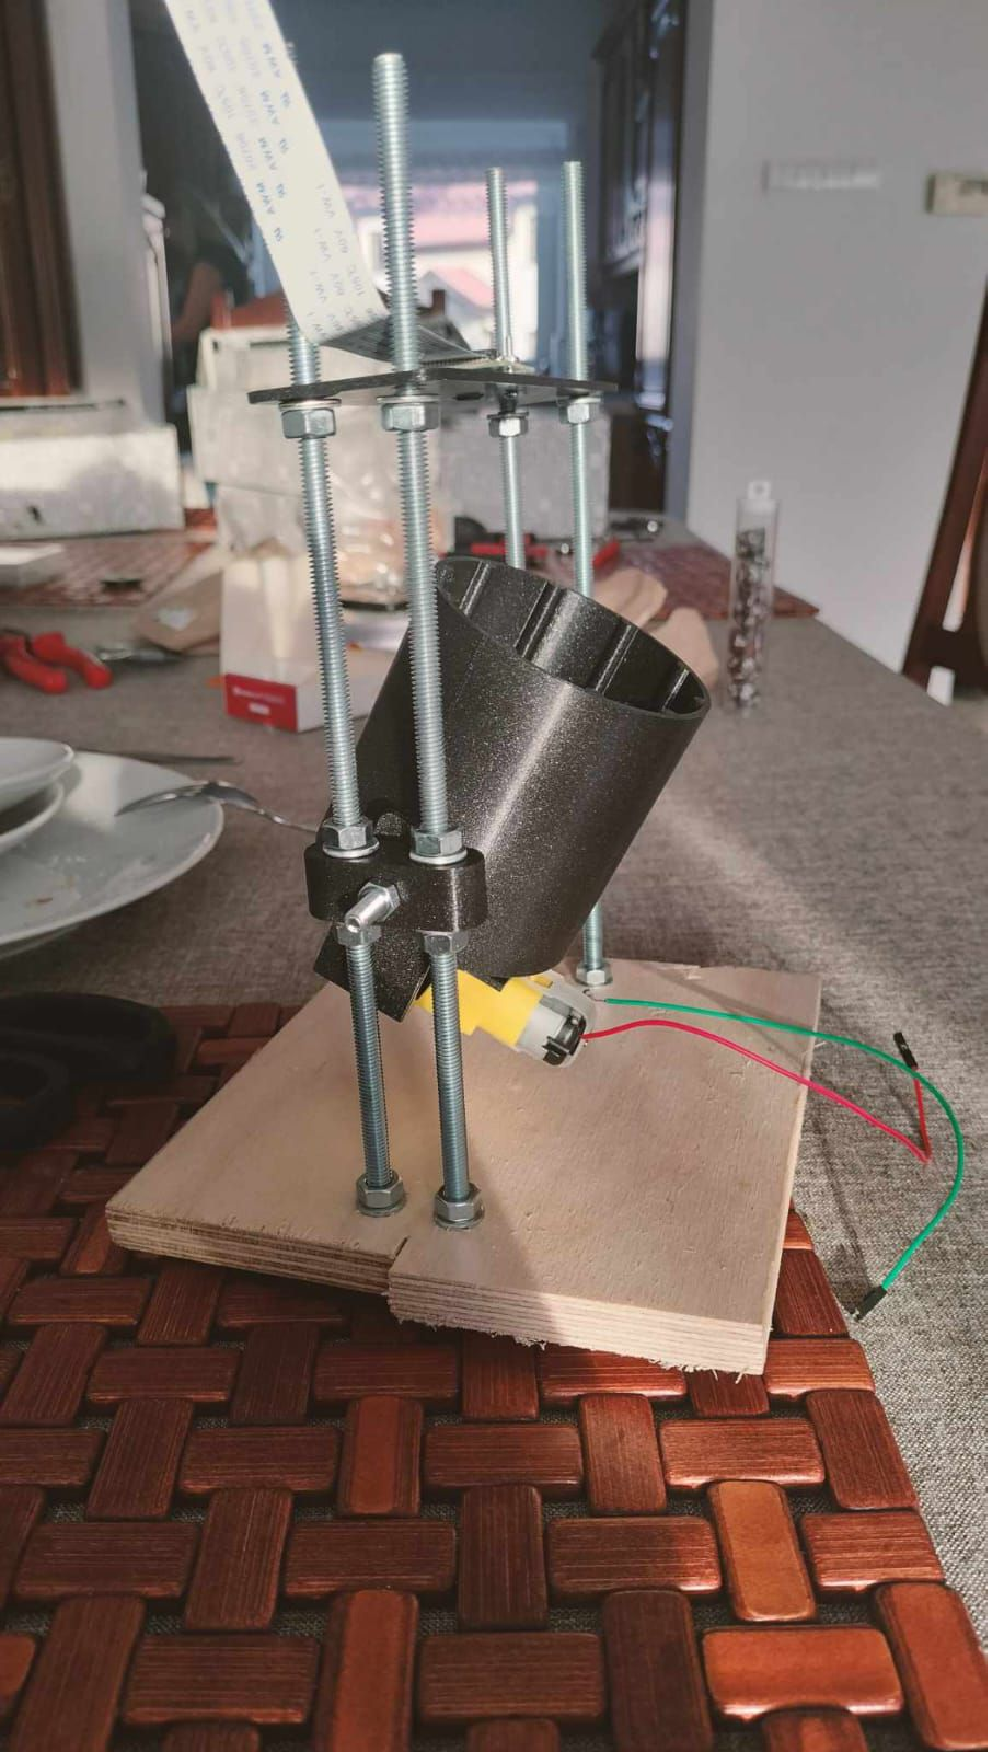
\includegraphics{./figures/pierwszy.pdf} % dostosowanie szerokości
% \end{figure}

Po pierwszych testach okazało się, że niezbędny do uzyskania zamierzonego efektu będzie mechanizm, który będzie 
wychylał cały kubek wraz z silnikiem, który odpowiada za jego obrót. Z początku planowano wykorzystanie prostogo
serwomechanizmu jednak to rozwiązanie odrzucono, ponieważ większość dostępnych serwomechanizmów, które byłyby odpowiednie w tym celu ma
ograniczony ruch do $180^{\circ}$ lub $360^{\circ}$ a to limitowałoby możliwości mechanizmu służącego do wychylania kubka.
Ostatecznie w tym celu wybrano mały silnik krokowy z wystarczającym momentem obrotowym (34.3mN.m). Silnik ten obraca 
układem dwóch kół zębatych 1:2 dzięki czemu silnik ma jeszcze większy zapas momentu obrotowego. Dzięki takiemu rozwiązaniu silnik
nie pracuje na granicy swoich możliwości co zapewni jego długi okres eksploatacji. 

Podczas testów pierwszej wersji robota wykorzytującej obrotowy kubek powstał pomysł alternatywnego rozwiązania.
Rozwiązanie to implementuje inne podejście do rzutu kością. Zamiast obracać cały kubek a dodatkowo wyhylać go,
wykorzystany został trwale zamontowany kubek na którego dnie znajduje się śmigło, które podcina leżącą na dnie kość.
Takie rozwiązanie znacząco upraszcza cały mechanizm robota a dodatkowo bardzo przyspiesza proces losowania liczby.

Przy projektowaniu drugiego wariantu robota zostal wykorzystany ten sam stelaż złożony z metalowych prętów co w 
pierwszym wariancie. Na drukarce 3d wydrukowano dodatkowe części niezbędne do realizacji tego wariantu.
Zaprojektowano i wydrukowano nowy kubek, śmigło oraz mocowanie dla silnika. Kubek został przystosowany do montażu 
silnika prądu stałego oraz śmigła. 

%tu kłamie bo jeszcze nie zrobilem tego
W obu wariantach dużym problemem był słaby obraz z kamery. W tym celu zaprojektowano system oświetlenia składający się z diod
LED sterowanych za pomocą układu ULN2803A Darlington. Dzięki temu wnętrze kubka stało się dużo jaśniejsze co pozwala kamerze na
robienie zdjęć o wystarczająco dobrej jakości dla zamierzonego celu. 





%%%%%%%%%%%%%%%%%%%%%%%%%%%%%%%%
%TODO
%1. oświetlenie 
%2. dodać wiecej informacji
%3. ostateczny projekt robota
%4. całe mnóstwo poprawiania i dopracowywania tego tekstu
%5. dodać zdjęcia/modele
